\documentclass[onecolumn, 12pt]{report}
\usepackage{hyperref,mathtools,amssymb}
\usepackage{cite}
\usepackage{graphicx}
\usepackage{xcolor}
\usepackage{subcaption}
\usepackage[margin=0.75in]{geometry}

\title{ERCAP Proposal: rotating bosons via CL with AMReX}
%\subject{Many-Body Quantum Mechanics}
\author{Casey Berger, Don Willcox}
\date{\today}

\newcommand{\note}[1]{{\color{red} \bf[NOTE: #1]}}
\newcommand{\etal}{{\it et al.}}
\newcommand{\beq}{\begin{equation}}
\newcommand{\eeq}{\end{equation}}
\newcommand{\bea}{\begin{eqnarray}}
\newcommand{\eea}{\end{eqnarray}}

\newcommand{\MarginPar}[1]{\hspace{1sp}\marginpar{\tiny\sffamily\raggedright\hspace{1sp}{\color{blue}#1}}}

\def\CP{{\mathcal P}}
\def\CC{{\mathcal C}}
\def\CH{{\mathcal H}}
\def\CW{{\mathcal W}}
\def\CO{{\mathcal O}}
\def\CZ{{\mathcal Z}}
\def\CD{{\mathcal D}}
\def\del{{\nabla}}

\newcommand*\dif{\mathop{}\!\mathrm{d}}

\begin{document}
\section{Project Description}
TO DO
\begin{itemize} 
	\item Add references
	\item Fill in all notes
\end{itemize}

\note{Add big picture paragraph:

This project aims to...

The CL method allows us to overcome difficulties by

I have developed and previously tested a code to do this

Add plan for publishing: series of papers. Add a few sentences on what you've done so far and what remains to be done.

Scaling studies have been performed and tests have been done to elucidate the computational needs of this problem. We request 30Mh from NERSC in 2021 in order to complete this calculation.}

\MarginPar{Oh, I forgot! Also we'll need to estimate our archival storage requirements, similarly to the time request, by estimating the total size of plotfile data all of the simulations will produce.}

\subsection{Motivation}
Quantum many-body systems are foundational to a huge range of physical scenarios, from very small scales to very large ones. The implications of improving our theoretical understanding of these systems include advancing the development of novel quantum materials, shedding light on the relationship between the nuclear interaction and atomic stability, and help us see more clearly into the first moments of the universe. Unfortunately, very few of these systems are accessible using analytical methods, and those which can be calculated computationally often have limitations that prevent us from exploring some of the most interesting regimes. This system which this project intends to study is that of the rotating bosonic superfluid. Understanding rotating bosons can shed light on a range of physical systems, from rotating nuclei to pulsars. Experiments using ultracold atomic gases confined with optical traps and stirred with a magnetic field have studied these systems in depth and have revealed much about the behavior of rotating bosonic systems, including the spontaneous formation of vortices. Unfortunately, these behaviors do not yet have a full theoretical description.

The use of computational methods have provoked great advances in our understanding of these fundamental systems. The advent of Quantum Monte Carlo (QMC) methods brought on huge leaps in our ability to tackle questions in nuclear theory, condensed matter physics, cosmology, and more areas where the complexity of the many-body Schr\"{o}dinger equation made analytical evaluation impossible. Quantum Monte Carlo allows for the statistical evaluation of the path integral, by treating the weight of each potential path as a probability distribution and sampling from that distribution using a Markov chain method such as the Metropolis Algorithm. 

However, the computational intensity of many quantum problems scales exponentially with the size of the system, meaning that many of the systems we most wish to examine remain inaccessible to us due to limitations in computational power. One of the largest sets of these systems are those which suffer from the sign problem. This is part of a larger group in computer science known as NP-hard problems, for which no general solution is expected to exist (although it remains a topic of ongoing research). In the case of many-body quantum physics, the sign problem  arises when the weight in the path integral is complex or oscillates between positive and negative values. In this case, the crucial step for the QMC approaches which have driven much of our advancement in computational quantum physics becomes invalid. It is exactly this challenge which has prevented us from performing a full quantum calculation of rotating bosonic superfluids, as the weight in the path integral is complex.

This challenge requires innovative methods, rather than straightforward increases in hardware. Exact solutions to the many-body Schr\"{o}dinger equation require more computational resources than exist, and so creative and intelligent alternatives must be developed. The method this project uses is known as the Complex Langevin (CL) method, and allows for a numerical evaluation of the path integral without sampling from a probability distribution, thereby circumventing the sign problem present in QMC treatments of these systems. 


\section{The physical system and the algorithm: complex Langevin and AMReX}
Rotating bosonic systems can be described using the path-integral formulation:
%
\beq
\CZ = \int \dif \phi e^{-S[\phi]}
\eeq
%
with the action in $2+1$ dimensions given by
%
\beq
S = \int \dif x \dif y \dif\tau \left[ \phi^{*}\left( \partial_{\tau} - \frac{\del^{2}}{2m} - \mu  - \frac{m}{2} \omega_{\text{trap}}^{2}(x^{2}+y^{2})- i \omega_{z}(x \partial_{y} - y\partial_{x})\right)\phi + \lambda (\phi^{*} \phi)^{2}\right],
\eeq 
%
where our scalar fields are functions of space and euclidean time, $\phi(x,y,\tau)$. The bosonic fields are complex scalar fields, and the addition of a rotational term in the action makes the system irretrievably complex. In order to treat this action composed of complex-valued fields, we use the CL method.

Complex Langevin is a stochastic method for treating field-theoretical models with a complex action. It extends the well-established Langevin method to complex-valued fields, evolving those fields in a fictitious time called Langevin time, resulting in a set of field values distributed with the appropriate weight $e^{-S}$, from which quantities of interest can be computed via a simple statistical average. This treatment has been shown to be successful in toy models for finite quark density QCD~\cite{BergerCLReview} as well as in low energy atomic systems such as the polarized unitary Fermi gas~\cite{BergerCLReview}. 

The complex Langevin method complexifies the fields, $\phi$, and evolves the complexified components of the fields according to a set of coupled stochastic differential equations, which include a drift function derived from the action of the system and a gaussian-distributed noise term to satisfy the stochastic properties. 

%
\note{Add a very loose, schematic description of the discretization and the process which leads to the algorithm}
%

From these complexified field components, quantities of interest (``observables") can be calculated and saved. The algorithm for a numerical study of rotating bosons with CL is shown in Fig.~\ref{Fig:Algorithm}.
%
%\vspace{-3mm}
\begin{figure}[h]
\centering
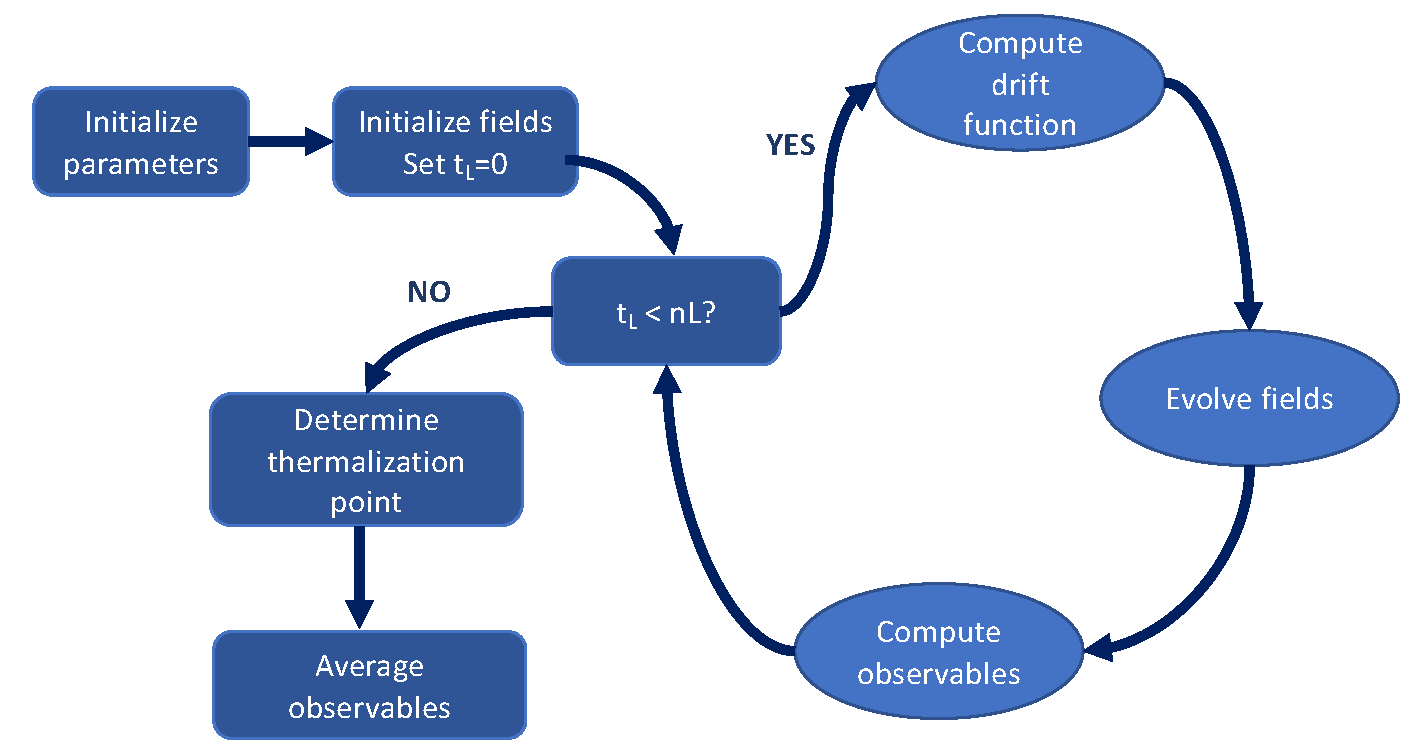
\includegraphics[width=0.6\textwidth]{./algorithm.pdf}
\caption{\label{Fig:Algorithm} Flow chart of the complex Langevin algorithm for rotating bosons.\vspace{-3mm}}
\end{figure}
%\vspace{-3mm}
%
The field components are defined on a euclidean spacetime lattice, and the evolution is performed for hundreds of thousands of steps in Langevin time in order to generate enough samples to calculate observables with good statistical properties. The code for this project is written in C++ and utilizes the AMReX framework. The adaptive mesh framework in AMReX will allow us to use a nonuniform mesh to calculate the field values, which enables more efficient use of computing resources. As the lattice size grows, we concentrate our resolution in the center of the lattice, where the interesting physics will be confined due to the presence of the harmonic traps, which reduce the presence of the fields rapidly to zero outside a narrow region in the center of the trap.

In order to explore the regions of interest, we must run this calculation on very large lattices, which requires large amounts of computational power. \note{add a few lines about computational limitations}

\subsection{Connection to DOE Office of Science}
Previous work on this topic has been supported by the Department of Energy Computational Science Graduate Fellowship. Current work is supported under a grant from the Exascale Computing Project (ECP) for Application Development for Lattice Gauge Theory. This work is similar to the work supported by ECP, but is more exploratory work for applications of this method to other systems of interest.

\section{Scaling and Performance}

This code uses AMReX, a high-performance AMR library developed at LBNL and
funded as an ECP Co-Design Center. We use AMReX data structures to discretize
the spacetime lattice upon which the fields are defined, distribute the lattice
across MPI, and implement local parallelism for CPU, KNL, or GPU-based
platforms while maintaining performance portability.

While each step in Langevin time must be performed sequentially, the spacetime
lattice can be updated at each of these Langevin steps in a naively parallel
fashion. We divide the lattice into boxes (or grids) distributed across MPI
ranks, so to advance the solution we first fill ghost cells throughout the
domain to support the nearest neighbor sums that appear in the drift function.
Next, we perform the drift function calculations and Langevin update - these
are entirely local operations for each MPI rank. We parallelize this local work
using OpenMP with logical tiling for CPUs or KNL to maintain cache efficiency.
Alternately, when running on GPUs, we transparently launch CUDA kernels and
disable logical tiling to ensure maximum kernel occupancy.

We also efficiently calculate observables at runtime, which requires summing
terms across the entire lattice for density, field modulus, circulation, and
other quantities of interest. On each MPI rank, the observables are first
calculated for local grids via OpenMP sum reductions (or using CUDA atomics for
GPUs). We then combine partial sums across the lattice using all-to-one MPI
reductions. In Fig.~\ref{Fig:GPUScaling} we compare strong scaling curves on
the Cori GPU development system for a $1024^3$ lattice for a run without
observables (orange) and a run where we calculate observables every 10 Langevin
steps (blue). We demonstrate that although the additional computation and
communication for observables requires about twice as much walltime, our
reduction strategy yields nearly ideal strong scaling efficiency.

Our parallel implementation uses AMReX abstractions developed for performance
portability on heterogeneous architectures. We have developed and tested it on
the NERSC Cori KNL nodes and Cori GPU development platform. We present scaling
studies on Cori KNL in Fig.~\ref{Fig:KNLScaling} showing good strong scaling
efficiency up to 10,000 KNL cores for a moderately sized domain of $512^3$
lattice sites. In Fig.~\ref{Fig:GPUScaling} we show excellent strong scaling on
the Cori GPU system using up to 96 GPUs for moderate and larger ($1024^3$)
domains.  We currently perform well on the Cori KNL platform and are already
poised to take full advantage of GPUs at NERSC once the Perlmutter system comes
online.

\note{Message: you give us time on your system and we will use it efficiently.}

\MarginPar{undecided about including a sentence about I/O, maybe it's worth
pointing out that we can use the Cray parallel HDF5 module on Cori in addition
to the native AMReX format, but I/O timing measurements would really help make
that point, we don't have those yet...}

%
%\vspace{-3mm}
\begin{figure}[h]
\centering
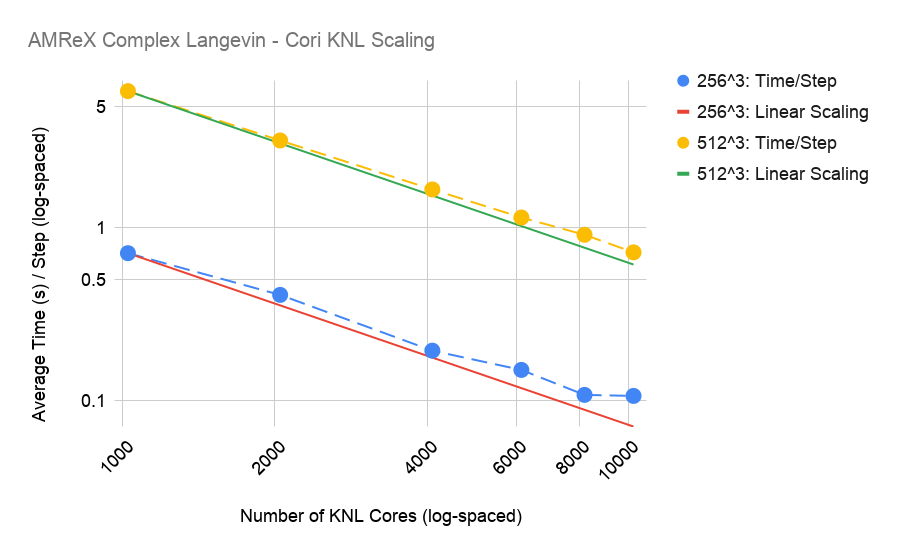
\includegraphics[width=0.6\textwidth]{./AMReX_Complex_Langevin_Cori_KNL_Scaling.png}
\caption{\label{Fig:KNLScaling} Strong scaling for AMReX Complex Langevin on Knights Landing accelerators. These runs were performed with box sizes of $32^3$, 4 MPI tasks per node, and 16 OpenMP threads/MPI task.\vspace{-3mm}}
\end{figure}
%\vspace{-3mm}
%

%
%\vspace{-3mm}
\begin{figure}[h]
\centering
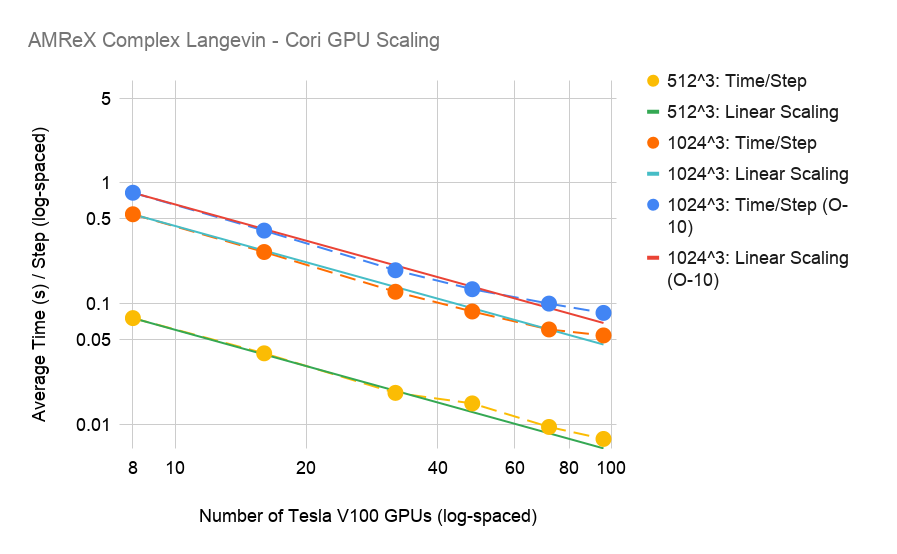
\includegraphics[width=0.6\textwidth]{./AMReX_Complex_Langevin_Cori_GPU_Scaling.png}
	\caption{\label{Fig:GPUScaling} Strong scaling for AMReX Complex Langevin on NVIDIA Tesla V100 GPUs. These runs were performed with box sizes of $32^3$ and $128^3$ for the $512^3$ and $1024^3$ domains, respectively, using 1 MPI task per GPU and no logical tiling. For the run labeled ``O-10'' we calculate observables every 10 Langevin steps, otherwise we turn off observables to measure performance for the Langevin advance alone.\vspace{-3mm}}
\end{figure}
%\vspace{-3mm}
%


\note{Describe what sort of data you will need to take. Relate your time estimates}

\note{I will need to do some testing on these larger lattices in order to determine the correct balance of trapping frequency, lattice size, and interaction strengths. Once these parameter values are set, we will need to collect on the order of 100 data points on each lattice (varying the chemical potential and the rotation frequency). We also wish to extend our time domain and examine the effect of decreasing the temperature on the formation of vortices.}


\end{document}
